\documentclass{article}
\usepackage[spanish]{babel}
\usepackage[utf8]{inputenc}
\usepackage{tikz}
\usepackage{johd}

\title{Tema 2. Protocolo HTTP}

\author{José Antonio Fajardo Naranjo \\
	\small
	\tt{fajardonaranjoja@gmail.com} \\
	\date{}
}

\begin{document}
	\maketitle
	\begin{abstract} 
		\noindent Estos apuntes pertenecen al tema 2 de la asignatura Desarrollo Web en entorno servidor impartida en el 2ndo curso de FPGS de Desarrollo de aplicaciones web en el IES Martín Rivero durante el curso 2023/2024.
	\end{abstract}
	\newpage{\ }
	\tableofcontents
	\newpage{\ }
	\thispagestyle{empty}
	
	


	\section{Introducción}
	
	\paragraph{}El protocolo HTTP busca la simpleza y la eficacia para el intercambio de documentos. Aunque su uso principal es el intercambio de los documentos de hipertexto se puede usar para transferir otro tipo de elementos.
	
	\subsection{Funcionamiento}
	
	\paragraph{}El principio en el que se basa este protocolo es el tándem pregunta/respuesta. El cliente genera una pregunta con la forma de una petición HTTP que contiene, al menos, los datos que permiten identificar el recurso que le ha sido solicitado por el cliente. Esta petición no es más que un bloque de texto que viaja del cliente al servidor. Se compone de dos partes separadas por una línea en blanco (retorno de carro o salto de línea). La primera parte es la cabecera de la petición HTTP, que es obligatoria, mientras que la segunda es el cuerpo, que es opcional, dependiendo su aparición del tipo de petición HTTP. La línea en blanco ha de aparecer siempre, siendo completamente \textbf{obligatoria}. La respuesta mantiene el mismo formato de las peticiones.
	
	\paragraph{}Una respuesta HTTP sólo existe si se ha enviado previamente una petición HTTP al servidor, no tomando este último la iniciativa de enviar datos que no han sido solicitados por el cliente (con la tecnología de los \textbf{WebSockets} esto no es necesario, los servidores actualizan en tiempo real sin necesidad de petición).
	
	\paragraph{}El protocolo TCP se utiliza para el transporte de los bloques de texto de petición y respuesta HTTP. Por defecto, esta conexión mediante TCP se establece para cada par petición/respuesta. Sin embargo, la versión 1.1 propone una solución para transportar varios pares petición/respuesta con la misma conexión TCP. A continuación, encontramos el ejemplo utilizado en clase de paquete capturado.
	
	\begin{figure}[H]
		\centering
		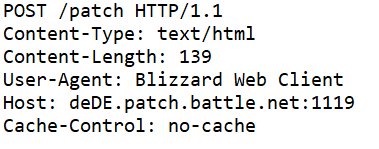
\includegraphics[scale=0.5]{images/peticionhttp.PNG}
		\caption{\label{fig1}Captura de una petición HTTP}
	\end{figure}
	
	\begin{figure}[H]
		\centering
		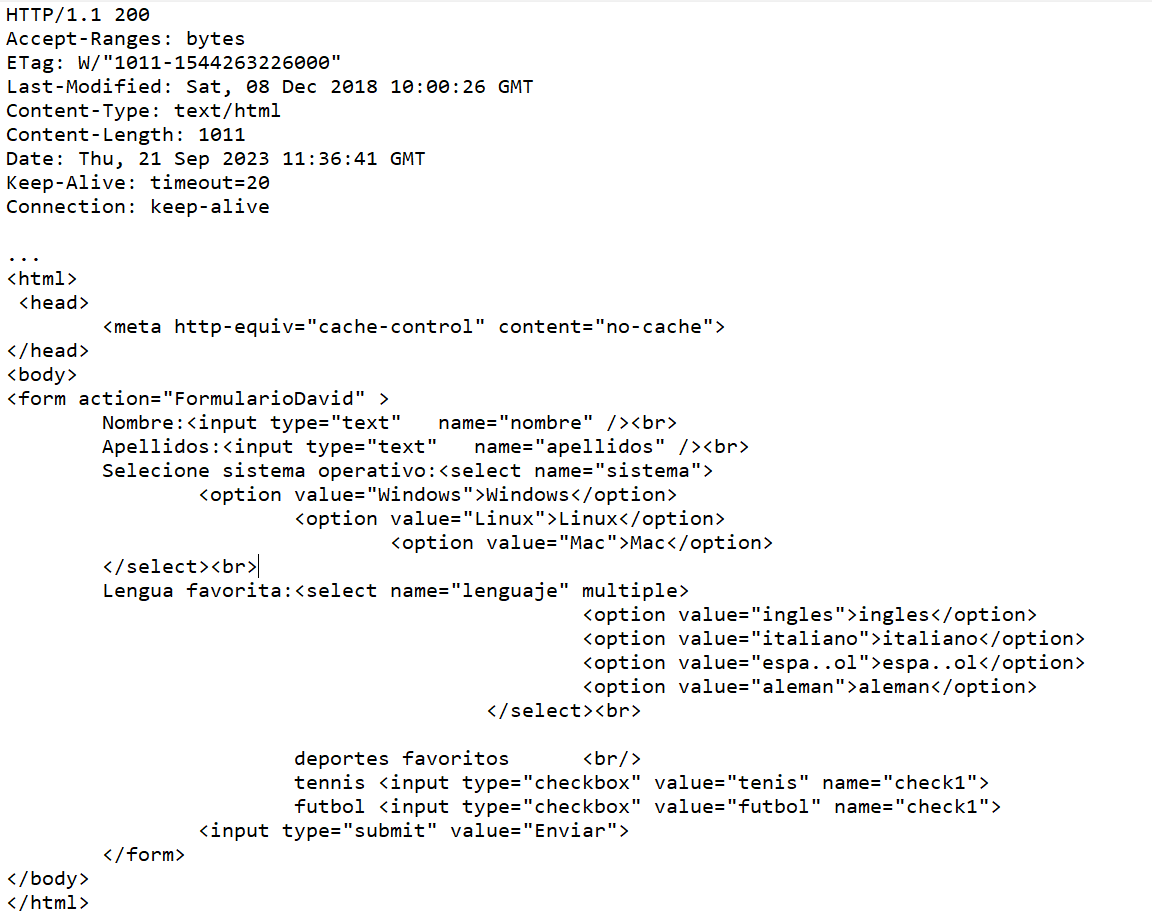
\includegraphics[scale=0.5]{images/respuestahttp.png}
		\caption{\label{fig2}Captura de una respuesta HTTP}
	\end{figure}
	
	\subsection{Las URL}
	
	\paragraph{}Las URL (Uniform Resource Locator) permiten localizar los recursos que se desean recuperar mediante peticiones HTTP. Se componen de una cadena de caracteres de cinco campos. Se ha de seguir el siguiente formato:
	
	\begin{center}
			\texttt{protocolo://identificador del servidor:número de puerto/recurso?parámetros}
	\end{center}
	
	\begin{itemize}
		\item Protocolo: indica el protocolo utilizado para el acceso al recurso. Nosotros usaremos HTTP aunque hay otros como FTP o mailto.
		\item Identificador del servidor: esta parte permite localizar el servidor en la red. Normalmente es el FQDN (Fully Qualified Domain Name), el nombre de dominio del servidor, que no da lugar a ambigüedades. Se tiene que transformar en la dirección IP para que el protocolo TCP pueda establecer una conexión con el servidor, de lo cual se encarga un servidor DNS (Domain Name System). Se puede usar una IP en la URL pero es más sencillo el FQDN.
		\item Número de puerto: este dato es el número de puerto TCP con el que se debe establecer la conexión. Este número funciona para que el protocolo TCP identifique una aplicación particular en una máquina. Este sistema permite el alojamiento de más de una aplicación por servidor. El puerto 80 es el que se asigna por defecto al protocolo HTTP.
		\item Recurso: esta parte de la URL permite determinar el recurso que se desea obtener. Puede estar compuesto por varios elementos separados por el carácter.
		\item Parámetros: son los datos que pasamos cuando la petición HTTP se hace, por ejemplo, sobre un recurso dinámico. Aparecen de la forma nombreDeParam=valorDeParam. Con el carácter \& se pueden separar estos parámetros.
	\end{itemize}
	
	\paragraph{}A continuación se muestran equivalencias entre los caracteres y su valor en ASCII, ya que algunos caracteres tienen una función en las URL:
	
	\begin{table}[H]
		\centering
		\begin{tabular}{|l|l|}
			\hline
			\multicolumn{1}{|c|}{\textbf{Carácter}} & \multicolumn{1}{c|}{\textbf{Codificación}} \\ \hline
			Espacio                                 & \%20 o a veces +                           \\ \hline
			"                                       & \%22                                       \\ \hline
			\%                                      & \%25                                       \\ \hline
			\&                                      & \%26                                       \\ \hline
			+                                       & \%2B                                       \\ \hline
			.                                       & \%2E                                       \\ \hline
			/                                       & \%2F                                       \\ \hline
			?                                       & \%3F                                       \\ \hline
			'                                       & \%60                                       \\ \hline
		\end{tabular}
	\end{table}
	
\end{document}